\section*{Results}

\subsection*{Empirical delays impose strong low-pass filtering}
Figure~\ref{fig:intro} illustrates how delayed observation can fundamentally limit the temporal resolution of epidemic surveillance. We now ask whether this theoretical mechanism holds across published epidemiological delay distributions.


We evaluated the theoretical predictions using several published epidemiological delay distributions spanning both biological delays (exposure-to-onset) and surveillance delays (symptom-onset-to-report) (Fig.~\ref{fig:empirical-delay-identifiability}A,D). Together, these representative delays span diverse diseases, surveillance settings, geographic regions, and study periods, providing a broad test of whether the theoretical predictions hold across realistic epidemiological delay processes.

For each delay distribution \(g(\tau)\), we computed its frequency response \(\widehat G(f)\) and attenuation profile \(|\widehat G(f)|^2\). Despite their heterogeneous epidemiological origins, all representative delay distributions exhibited rapidly decaying frequency responses (Fig.~\ref{fig:empirical-delay-identifiability}B,E), confirming that the examined epidemiological delays consistently behave as low-pass filters.

Frequencies corresponding to weekly and sub-weekly variation (i.e., $f \geq 1/7$ cycles/day) fall in a strongly attenuated regime for many of the empirical delays. In some cases, especially for broader or more dispersed delay distributions, the power transmitted at weekly and faster frequencies is reduced by orders of magnitude relative to low-frequency components.

We next quantify how this attenuation translates into statistical detectability. The observed attenuation translates directly into a frequency-dependent detectability limit. Consider an upstream perturbation concentrated around a characteristic period \(T\), corresponding to frequency \(f_0 = 1/T\). Under the separability criterion derived in Methods, the contribution of this perturbation to downstream distinguishability is proportional to
\[
    J(f_0) 
    \;\propto\; 
    p^2 |\widehat G(f_0)|^2 
    \frac{|\Delta \widehat U(f_0)|^2}{N(f_0)} ,
\]
where \(N(f_0)\) is the effective noise level at frequency \(f_0\). The quantity
\[
\frac{|\Delta\widehat U(f_0)|^2}{N(f_0)}
\]
therefore represents the frequency-domain contrast-to-noise ratio, namely the upstream spectral contrast normalized by the effective downstream noise level.


For a fixed target testing-error level \(\alpha\), the model-specific non-identifiability threshold derived in the Methods implies that the minimum required contrast-to-noise ratio is
\[
    \left(\frac{|\Delta \widehat U(f_0)|^2}{N(f_0)}\right)_{\min}
    =
    \frac{\tau_{M,\alpha}}
    {p^2 |\widehat G(f_0)|^2},
\]
where \(M\) denotes the observation model and \(\tau_{M,\alpha}\) is the corresponding testing-error threshold. Throughout Fig.~\ref{fig:empirical-delay-identifiability}C,F, we illustrate this threshold under the negative-binomial observation model, for which \(\tau_{M,\alpha}=4(1-\alpha)^2\). 

Figure~\ref{fig:empirical-delay-identifiability}C,F visualize the minimum required frequency-domain contrast-to-noise ratio as a function of perturbation period \(T\). Under the same observation window, shorter-period perturbations require larger frequency-domain contrast-to-noise ratios, reflecting the progressively stronger attenuation of high-frequency components by the delay kernel. Lower conversion rates further amplify this effect: reducing \(p\) from \(1.0\) to \(0.2\) increases the detectability threshold by a factor of \(1/p^2=25\). Partial ascertainment therefore compounds the information loss caused by delay filtering.

Together, these results show that empirical epidemic delay distributions impose a finite temporal resolution limit on upstream inference. The key consequence is not simply that delays smooth the observed data, but that they make short-timescale upstream variation statistically difficult to distinguish from noise. Perturbations occurring over several weeks may remain visible after delay convolution, whereas weekly or sub-weekly fluctuations often require unrealistically large contrast-to-noise ratios to be identifiable. 

\begin{figure*}[h!]
    \centering
    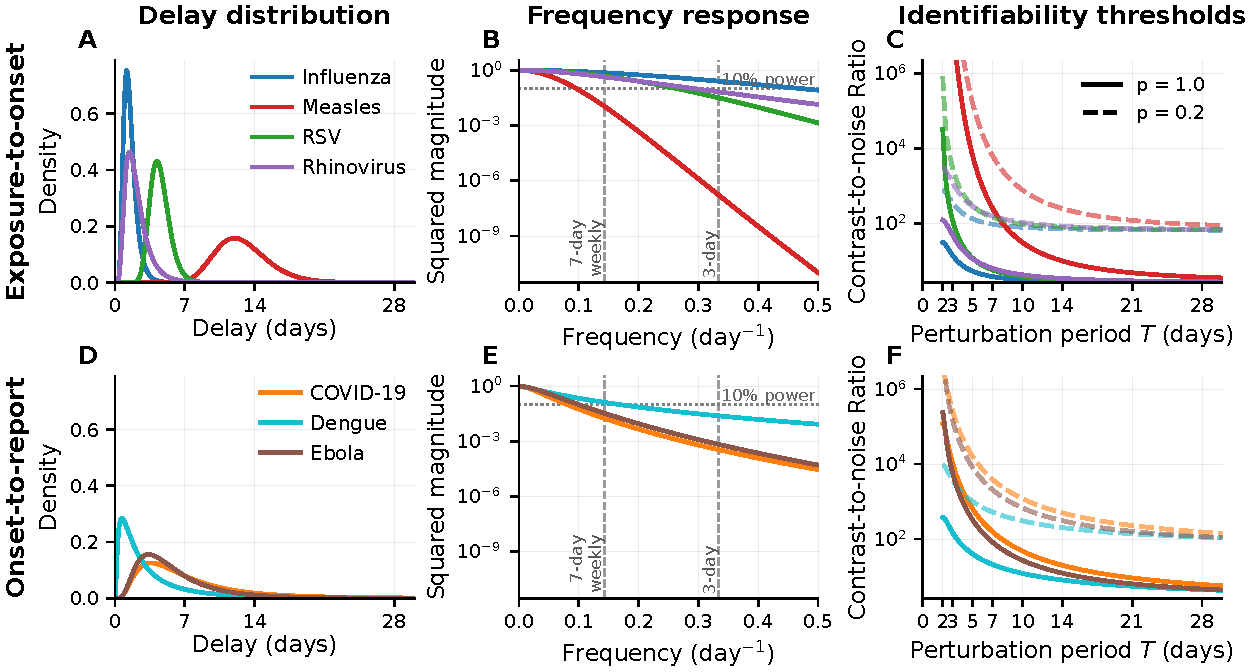
\includegraphics[width=\textwidth]{figs/empirical_delays_3x2_with_rmin.pdf}
    \caption{
    \textbf{Empirical epidemic delays impose a frequency-dependent limit on upstream identifiability.}
    (A,D) Representative published delay distributions for exposure-to-onset (\cite{lessler2009incubation}) and onset-to-report processes across multiple diseases (\cite{zhang2020evolving}, \cite{bastos2019modelling}, \cite{fang2016transmission}, \cite{hinch2024quantification}). (B,E) Corresponding squared magnitude \( |\widehat G(f)|^2 \) of the delay kernels. Vertical dashed lines indicate frequencies corresponding to 7-day and 3-day periods. The dotted horizontal line marks the 10\% power level. (C,F) Minimum required frequency-domain contrast-to-noise ratio needed for statistical distinguishability as a function of perturbation period \(T = 1/f\), derived from the separability criterion. Solid and dashed curves correspond to conversion rate \(p=1.0\) and \(p=0.2\), respectively.
    }
    \label{fig:empirical-delay-identifiability}
\end{figure*}




\subsection*{Spectral identifiability constrains epidemiological inference}

The practical consequence of non-identifiability is not simply that multiple upstream trajectories can explain the same downstream observations. Rather, whenever downstream data fail to identify part of the upstream process, reconstruction necessarily relies on information external to the data, including prior distributions, smoothness assumptions, regularization constraints, or mechanistic model structure \cite{kaipio2005statistical, stuart2010inverse, miller2022statistical}. These assumptions play an essential role in stabilizing ill-posed inverse problems. However, they also imply that weakly identified components of a reconstructed trajectory are determined jointly by the observed data and by the assumptions used to complete the inference problem. Our objective is therefore not simply to characterize uncertainty in reconstructed incidence curves, but to determine which epidemiological conclusions are actually supported by the information preserved in delayed and noisy observations.

To illustrate this mechanism without comparing specific reconstruction algorithms, we constructed frequency-constrained upstream trajectories from the same downstream COVID-19 incidence series. For each cutoff frequency \(f_c\), we estimated an upstream trajectory \(U^\star_{f_c}\) restricted to Fourier components satisfying \(f \leq f_c\), while requiring its delayed projection \(K U^\star_{f_c}\) to remain consistent with the same downstream observations (Methods; Appendix~\ref{sec:Appendix_S3}). We considered \(f_c = 1/35\), \(1/14\), and \(1/7\) cycles/day, corresponding to characteristic periods of 35, 14, and 7 days. These trajectories are not intended as alternative epidemiological models. Instead, they illustrate how progressively admitting higher-frequency structure changes the range of admissible reconstructions.

To visualize this uncertainty, we computed frequency-constrained non-identifiable perturbation bands around each reference trajectory. These bands consist of perturbations whose downstream effect remains below the non-identifiability threshold implied by the separability criterion \(J\) (Appendix~\ref{sec:Appendix_S3}). The resulting bands widened as progressively higher-frequency components were admitted, illustrating that the set of upstream trajectories compatible with the same downstream observations expands when weaker frequency constraints are relaxed (Fig.~\ref{fig:epi-features}A).

In practice, reconstructed incidence curves are rarely the final inferential target. Instead, they are commonly used to derive epidemiological quantities such as epidemic peak timing, peak magnitude, and short-term growth rates. To examine how spectral identifiability translates into epidemiological inference, we evaluated these three representative quantities across the admissible reconstruction family. For visualization, peak timing was expressed as the normalized location of the epidemic peak within the study period, and peak magnitude was normalized by the largest reconstructed peak across the admissible reconstruction family (Fig.~\ref{fig:epi-features}D).

Although all admissible reconstructions generated nearly identical downstream trajectories (Fig.~\ref{fig:epi-features}B), they did not support the same epidemiological conclusions. Epidemic peak timing and peak magnitude remained remarkably consistent across the reconstruction family (Fig.~\ref{fig:epi-features}D), whereas inferred seven-day growth-rate trajectories differed substantially (Fig.~\ref{fig:epi-features}C).

To understand this contrast, consider the definition of the seven-day log growth rate,
\begin{equation}
r_7(t)
=
\frac{1}{7}
\left[
\log\{U(t+7)+c\}
-
\log\{U(t)+c\}
\right],
\end{equation}

where \(c>0\) is a small numerical offset. 

Unlike peak timing or peak magnitude, the seven-day growth rate is computed from local temporal differences. Temporal differencing emphasizes short-timescale variation (Appendix~\ref{sec:Appendix_S3}), causing growth-rate estimates to depend disproportionately on high-frequency components of the reconstructed trajectory. Under delayed observation, these are precisely the components that are most strongly attenuated by the delay kernel and least constrained by the downstream observations.


Consequently, the differences in the inferred seven-day growth-rate trajectories (Fig.~\ref{fig:epi-features}C) cannot be attributed to the downstream observations alone. Rather, they arise from alternative completions of weakly identified high-frequency components that remain effectively unconstrained by the observed data. In this sense, short-term growth-rate estimates are determined jointly by the information contained in the observations and by the assumptions used to reconstruct the weakly identified portion of the upstream trajectory.


These results demonstrate that agreement in downstream goodness-of-fit does not imply equal support for all epidemiological conclusions. Reconstructions that are statistically indistinguishable at the observation level may nevertheless lead to different scientific inferences. Spectral identifiability therefore provides a principled way to distinguish quantities that are constrained by the information contained in delayed observations from those that depend primarily on assumptions introduced to resolve the weakly identified components of the inverse problem.

\begin{figure*}[!t]
\centering
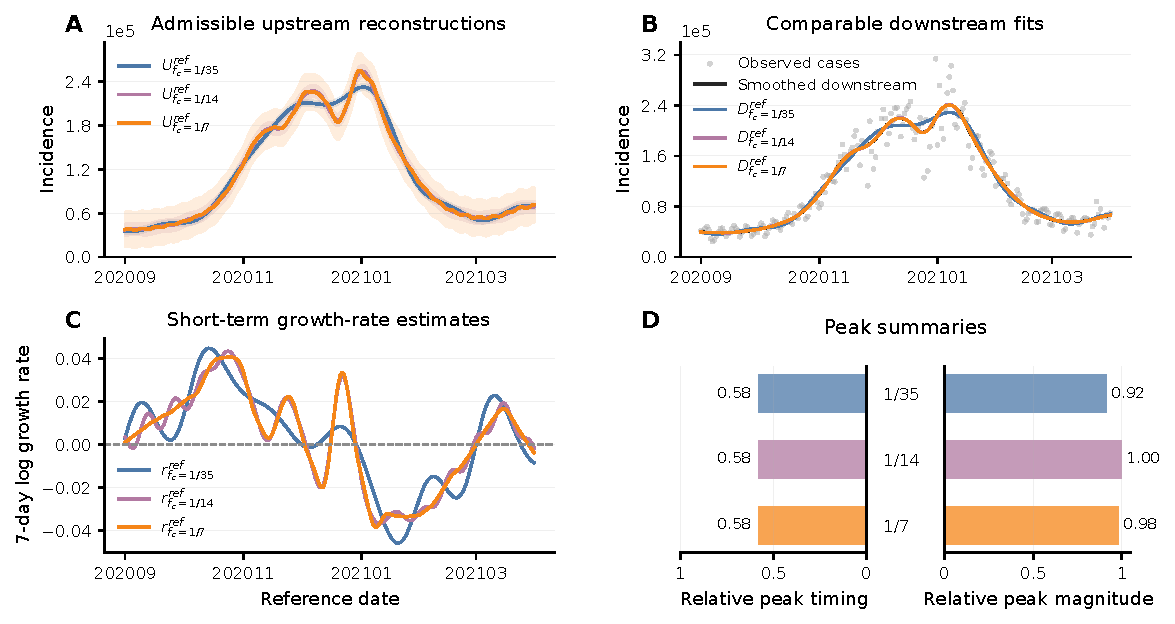
\includegraphics[width=\textwidth]{figs/epi_features_us.pdf}
\caption{
\textbf{Spectral identifiability constrains epidemiological inference.}
Frequency-constrained upstream reconstructions with cutoff frequencies
\(f_c=1/35\), \(1/14\), and \(1/7\) cycles/day.
(A) Admissible upstream reconstructions with corresponding non-identifiable perturbation bands.
(B) Delayed projections of the reconstructed trajectories together with the observed and smoothed downstream case series.
(C) Seven-day log growth rates derived from the reconstructed upstream trajectories.
(D) Relative peak timing and relative peak magnitude of the admissible reconstructions.
}
\label{fig:epi-features}
\end{figure*}






\subsection*{Event impacts form reference-conditioned low-separability landscapes}
Epidemiological events are often known independently of surveillance data. Mass gatherings are scheduled, temporary lockdowns are announced, and vaccination campaigns are documented administratively. The principal inferential question is therefore often not whether an event occurred, but which transmission impacts are distinguishable from competing explanations after delay filtering and observational noise. In particular, knowledge of an event's timing does not imply that its magnitude or temporal footprint can be uniquely recovered from downstream surveillance observations.

We characterized this uncertainty using reference-conditioned event-identifiability landscapes. For a specified reference event profile, these landscapes map alternative combinations of event duration and transmission impact according to their downstream separability after epidemic propagation, delay convolution, and observation noise. We considered three stylized event families representing common epidemiological perturbations: a transient increase in transmission associated with a mass gathering, a transient reduction associated with a temporary lockdown, and a gradual reduction associated with a vaccination rollout. The reference profiles corresponded to a 50\% peak proportional change in $R\_t$, with characteristic durations of 3, 10, and 60 days, respectively.

We represented each event through a transmission multiplier \(m(t;\theta)\) acting on a baseline reproduction-number trajectory,

\begin{equation}
R(t;\theta)
=
R_0(t)m(t;\theta),
\label{eq:event-Rt}
\end{equation}

where $\theta$ specifies the event duration (or rollout timescale) and the peak proportional change in $R_t$. The three transmission multipliers are summarized in Table~\ref{tab:event-models}. 

To examine how alternative event profiles propagate through epidemic dynamics and delayed observation, we conducted a controlled synthetic experiment. Synthetic epidemics provide a common baseline for comparison while avoiding the confounding effects of multiple overlapping drivers present in real outbreaks. Across all event classes, we used the same baseline epidemic trajectory, generation-interval distribution, renewal framework, delay kernel, conversion rate, and negative-binomial observation model with a common dispersion parameter. Within each event family, every candidate profile was generated by perturbing the same baseline epidemic through the same renewal process, so that differences in \(J_{\mathrm{event}}\) reflected only differences in the event profile under a common epidemic setting. Complete simulation details are provided in Appendix~\ref{sec:Appendix_S4}.

Incidence was generated through the renewal equation,

\begin{equation}
U(t;\theta)
=
R(t;\theta)
\sum_k w_k U(t-k;\theta),
\label{eq:event-renewal}
\end{equation}

and mapped to the downstream mean through the same delay kernel used throughout the analysis, where \(w_k\) denotes the generation-interval distribution.

\begin{table*}[t]
\centering
\small
\caption{
\textbf{Stylized event models used in the event-impact analysis.}
The parameter \(a\) denotes the peak proportional change in \(R_t\), and
\(\tau\) controls the event duration or rollout timescale.
}
\label{tab:event-models}

\begin{tabular}{lll}
\toprule
Event type &
Transmission multiplier &
Reference profile
\\
\midrule

Mass gathering
&
\(
1+a\,h_{\tau}(t-t_0)
\)
&
50\% increase, 3-day duration
\\[5pt]

Temporary lockdown
&
$
1-a\,h_{\tau}(t-t_0)
$
&
50\% reduction, 10-day duration
\\[6pt]

Vaccination rollout
&
$
1-a\,C_{\tau}(t)
$
&
50\% reduction, 60-day rollout
\\

\bottomrule
\end{tabular}

\vspace{1mm}

\raggedright
\footnotesize
The event window $h_{\tau}(t-t_0)$ is normalized to attain a maximum of one and is localized around the known event time $t_0$. The rollout curve $C_{\tau}(t)$ increases monotonically from zero to one over a timescale controlled by $\tau$.
\end{table*}

For a specified reference event \(\theta^\ast\), we compared each candidate profile \(\theta\) through the induced upstream contrast
\begin{equation}
\Delta U(t;\theta,\theta^\ast)
=
U(t;\theta)-U(t;\theta^\ast),
\end{equation}

and quantified its downstream separability using the spectral functional

\begin{equation}
J_{\mathrm{event}}(\theta,\theta^\ast)
=
\int
\frac{|p\widehat G(f)|^2
\left|
\Delta \widehat U(f;\theta,\theta^\ast)
\right|^2}
{N(f)}
\,df.
\label{eq:Jevent}
\end{equation}
We set \(p=1\) in the controlled examples. The resulting landscape is necessarily reference-conditioned: changing \(\theta^\ast\) changes the position and geometry of its low-separability neighborhood, but not the procedure used to construct it.

\begin{figure*}[!tbp]
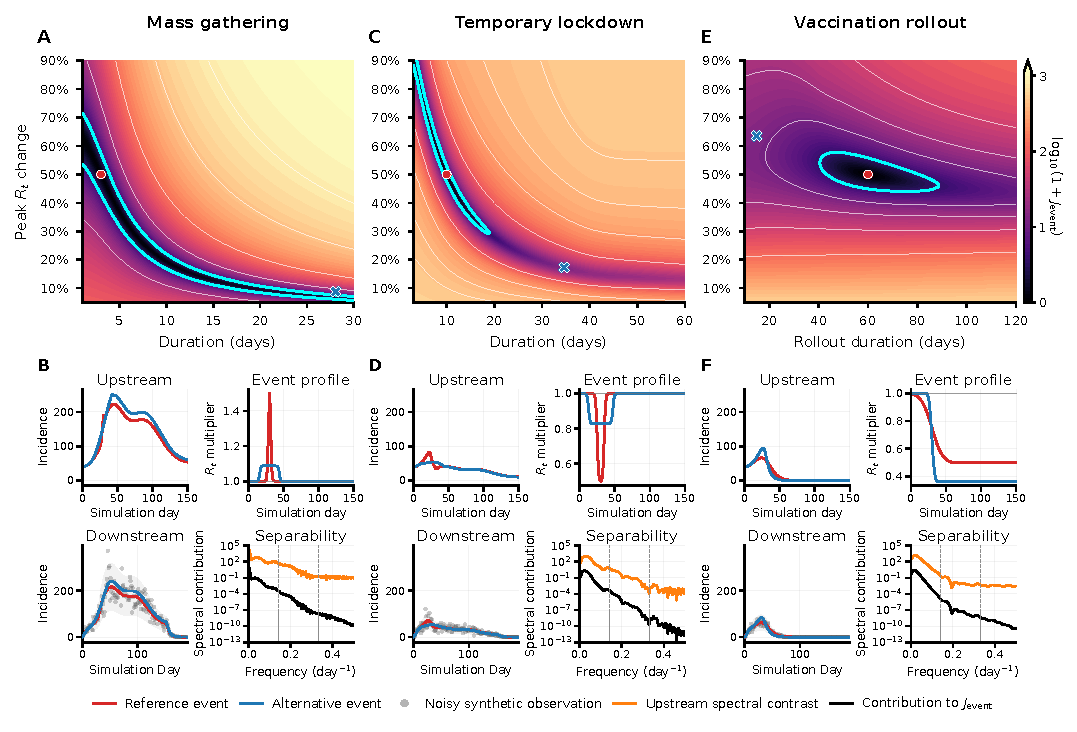
\includegraphics[width=\textwidth]{figs/event_controlled_synthetic_column_layout.pdf}
\caption{
\textbf{Event impacts occupy extended regions of weak downstream separability.}
Each column presents a reference-conditioned event-impact analysis for a mass gathering, temporary lockdown, or vaccination rollout.
(\textit{A,C,E}) Event-identifiability landscapes over duration, or rollout duration, and peak proportional change in \(R_t\). Color denotes \(\log_{10}(1+J_{\mathrm{event}})\), with darker regions indicating weaker downstream separation from the reference. Red circles mark the reference profiles. Cyan contours denote the sufficient non-identifiability boundary \(J_{\mathrm{event}}=4(1-\alpha)^2\), with \(\alpha=0.20\), under the negative-binomial observation model and effective noise scale defined in Methods. 
(\textit{B,D,F}) Propagation of each reference--alternative contrast through the inferential pipeline. Red and blue curves denote the reference and alternative profiles, respectively. Top left: upstream incidence. Top right: event-specific transmission multiplier. Bottom left: synthetic delayed downstream means and one noisy realization generated under the reference event, shown as gray points. Bottom right: upstream spectral contrast \(\left|\Delta\widehat U(f)\right|^2\) and its delay- and noise-weighted contribution to downstream separability,
\(\left|p\widehat G(f)\right|^2
\left|\Delta\widehat U(f)\right|^2/N(f)\).
Vertical dashed lines indicate frequencies corresponding to 7-day and 3-day periods. The zero-frequency component is included in \(J_{\mathrm{event}}\) but omitted from the displayed spectra.
}
\label{fig:event-impact}
\end{figure*}

The resulting landscapes reveal extended low-separability neighborhoods around each reference event rather than isolated identifiable parameter values
(Fig.~\ref{fig:event-impact}A,F,K). Within the cyan contour, the testing-error bound derived in Methods guarantees that every statistical decision rule has total error at least \(\alpha\) under the specified observation model. Candidate profiles in this region therefore cannot be reliably distinguished from the reference at the chosen error criterion. Beyond this boundary, separability increases continuously with \(J_{\mathrm{event}}\), but distinguishability is not guaranteed because the bound is sufficient rather than necessary.

The resulting landscapes reveal event-specific tradeoffs between transmission magnitude and event duration. For transient mass gatherings and temporary lockdowns, shorter but stronger perturbations can remain only weakly separated from longer but weaker perturbations. By contrast, vaccination rollout generates a more localized landscape because changes in rollout duration primarily alter lower-frequency epidemic dynamics. These geometries are not intrinsic properties of the event labels themselves; they emerge from the interaction among epidemic dynamics, delay filtering, and the spectral content of the induced transmission perturbation.

To illustrate the practical implications of these landscapes, we selected one representative alternative for each event class lying immediately outside the sufficient non-identifiability boundary while maximizing upstream trajectory contrast (Appendix~\ref{sec:Appendix_S4}). As shown in Fig.~\ref{fig:event-impact}B,C,G,H,L,M, the reference and alternative profiles produce visibly different transmission multipliers and upstream incidence trajectories. After delay convolution, however, much of this contrast is attenuated, and the resulting downstream means remain similar relative to observational variability. A single synthetic realization generated under the reference profile is visually compatible with both alternatives, illustrating that substantial ambiguity can persist even beyond the conservative theoretical boundary.

The spectral decomposition identifies the source of this ambiguity. At each frequency, the upstream contrast contributes to separability in proportion to
\[
\frac{|p\widehat G(f)|^2}{N(f)}
\left|\Delta\widehat U(f)\right|^2.
\]
The upstream contrast spectrum and its statistically usable downstream contribution can therefore differ sharply. Rapidly varying components are strongly compressed by delay attenuation and observational noise, whereas only contrasts overlapping sufficiently informative frequencies contribute materially to \(J_{\mathrm{event}}\). A substantial difference in upstream incidence consequently need not produce a correspondingly large amount of distinguishable downstream information.

Together, these results distinguish event occurrence from event-impact identifiability. Even when the timing and existence of an epidemiological event are known, delayed surveillance data may support a neighborhood of epidemiologically distinct transmission impacts rather than a unique estimate of event magnitude and duration. The event-identifiability landscape therefore provides a quantitative characterization of the competing transmission histories that remain only weakly separated from a specified reference under a given epidemic and observation model.